\chapter{Лабораторная работа 4}
\section*{Практическое задание}

Целью лабораторной работы №4 является отработка навыков использования программы Microsoft Project актуализации параметров проекта, ввода фактичесских данных для задач и просмотра отклонения от контрольного плана.

\textbf{Содержание проекта:} команда разработчиков из 16 человек занимается созданием карты города на основе собственного модуля отображения. Проект должен быть завершен в течение 6 месяцев. Бюджет проекта: 50 000 рублей.

Команда проекта состоит из 5 программистов (из них 1 ведущий), Web-дизайнера, системного аналитика, 5 наборщиков данных, 2 дизайнеров, технического писателя и медиа-корреспондента.

\subsection*{Задание 1}

Согласно полученному заданию была задана дата отчёта 15 мая (Проект, Состояние, Дата отчёта о состоянии):
\begin{figure}[h!]
	
\includegraphics[scale=1, center]{lab04_task1_1}
\end{figure}


\subsection*{Задание 2}

Все задачи со сроком завершения до 15 мая были отмечены как выполненные, со следующими исключениями: фактическая длительность задачи №5 была увеличена на 20 процентов (с 16 до 20 дней), дата завершения задачи №15 была установлена на 22 апреля, процент выполнения задачи №10 был установлен на 80 процентов.

Помимо этого использование сервера стало осуществляться на безвозмездной основе, а к затратам проекта прибавилось 3200 рублей согласно договору от 1 апреля об оказании организацией-партнёром сервисных услуг до конца проекта.

С 1 апреля ведущий программист был отправлен на курсы повышения квалификации на 2 недели, для этого была изменена доступность ресурса (в течении обучения доступность ведущего программиста снижена вдвое):

\begin{figure}[h!]
	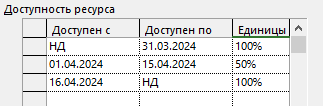
\includegraphics[scale=1, center]{lab04_task2_1}
\end{figure}

После прохождения курсов зарплата ведущего программиста была увеличена на 20 процентов:

\begin{figure}[h!]
	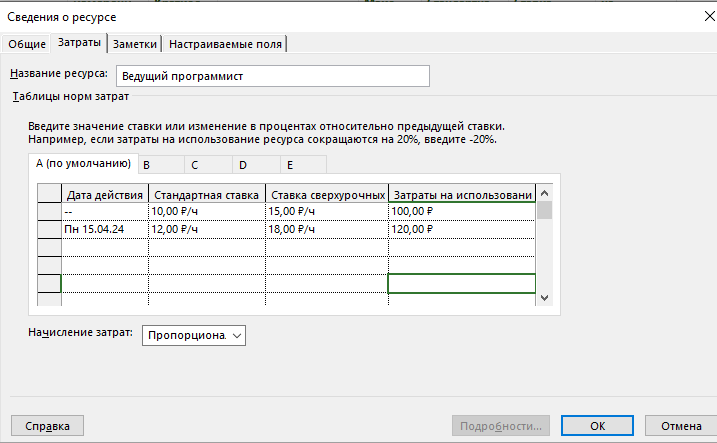
\includegraphics[scale=0.5, center]{lab04_task2_2}
\end{figure}

Также с 11 апреля совещания были заменены презентации, проходящие раз в 2 недели. Каждая презентация длится 2 часа, на ней присутствуют ведущий программист, мультимедиа-корреспондент, системный аналитик и Web-дизайнер. Также на каждой презентации используется по 0.5 пачки бумаги (1 пачка бумаги стоит 100 рублей), а также 6 бутылок воды (1 бутылка стоит 40 рублей).

Для этого была использована повторяющаяся задача со следующими параметрами:
\begin{figure}[h!]
	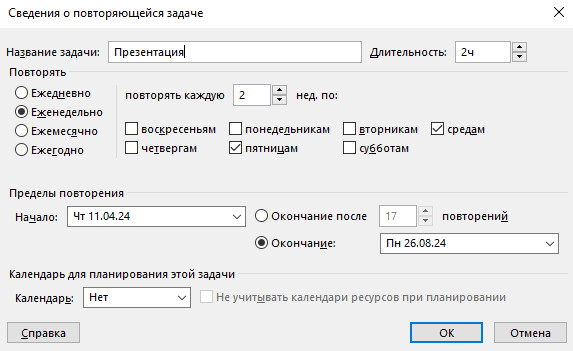
\includegraphics[scale=0.5, center]{lab04_task2_3}
\end{figure}

\begin{figure}[h!]
	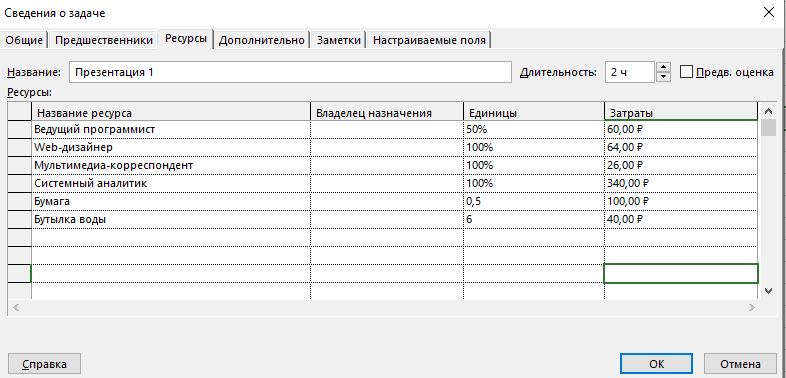
\includegraphics[scale=0.5, center]{lab04_task2_4}
\end{figure}

\subsection*{Задание 3}

После ввода фактических данных для задач дата окончания проекта сместилась с 18 августа на 16 августа, в то время как затраты по проекту уменьшились с 49 494 рублей до 47 725 рублей.

\subsection*{Задание 4}

Выведем линию прогресса:

\begin{figure}[h!]
	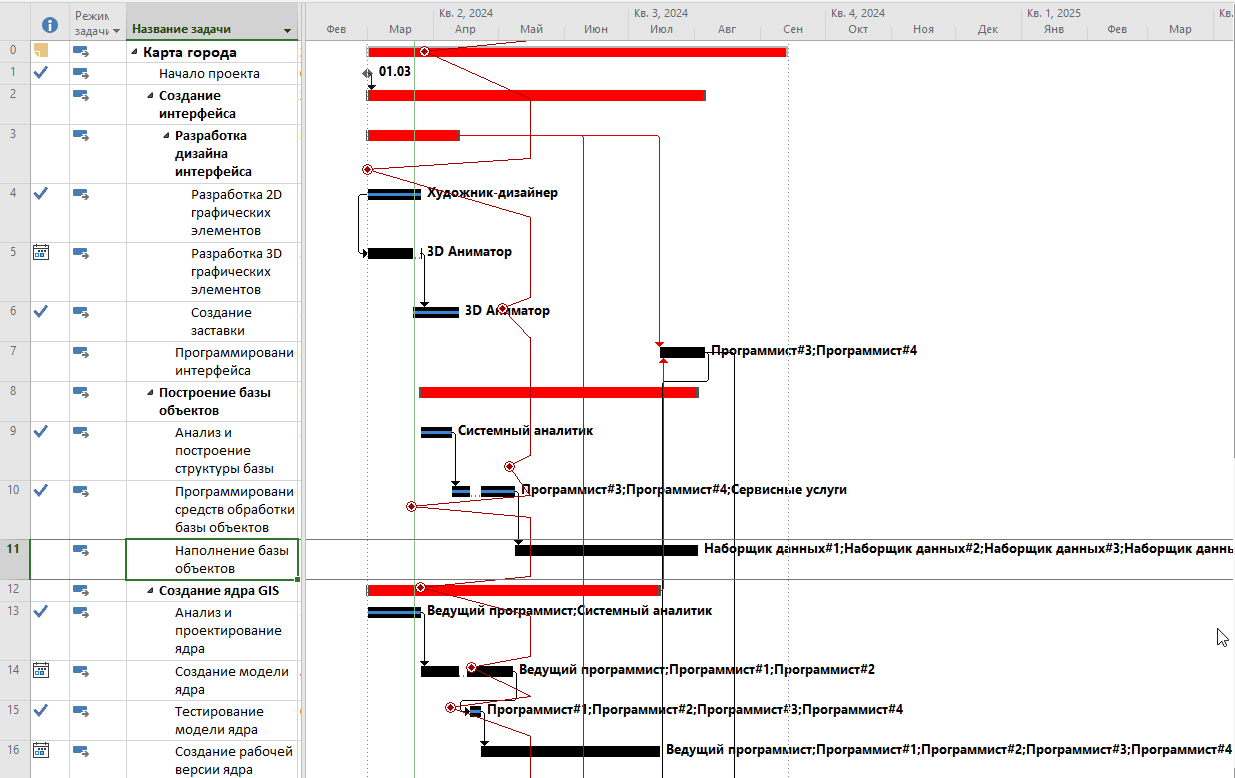
\includegraphics[scale=0.4, center]{lab04_task4_1}
\end{figure}

\begin{figure}[h!]
	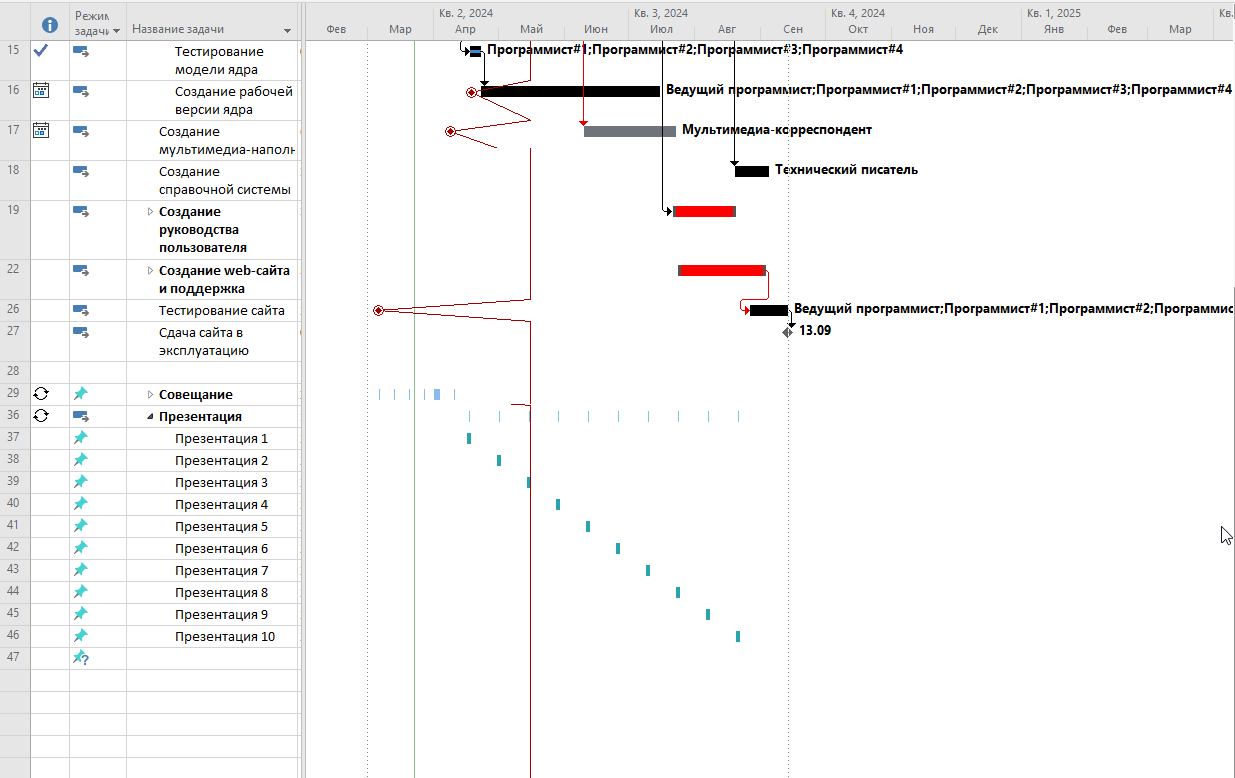
\includegraphics[scale=0.4, center]{lab04_task4_2}
\end{figure}

\clearpage

Задачи выполняются раньше, чем полагается, из-за того, что частые совещания, на которых должны присутствовать все специалисты, заменились более редкими презентациями, на которых присутствуют не все. 

Отметим, что присутствие ведущего программиста в период обучения компенсируется добавлением 1 рабочего часа в день его четырём подчинённым.

\subsection*{Задание 5}

Дата окончания проекта, а также затраты на проект находятся в требуемых пределах, временных и финансовых отклонений (в большую сторону) нет.

\section*{Заключение}

В ходе выполнения данной лабораторной работы были отработаны навыков использования программы Microsoft Project для оптимизации временных и финансовых показателей проекта.

В результаты затраты по проекту равны 47 725 рублей (укладывается в бюджет).
Посредством использования программистов в задаче по разработке ядра удалось снять нагрузку с вещущего программиста и уменьшить длительность проекта на месяц - теперь дата завершения проекта 16 августа (укладывается в срок).